\chapter{Laboratory Environment}\label{chap:config}
This chapter discusses the setup you will be using during this lab. Section \ref{sec:rasp} will explain what external hardware you will be going to use during this lab. Furthermore, this section will depict the way the hardware should be configured and which additional packages are required to guarantee correct functionality.Section \ref{sec:environment} will list the various operating systems that can be used in order to guarantee a correct and stable operation and communication with the hardware.\\ 

\section{External Hardware}
\label{sec:rasp}
\subsection*{Raspberry Pi}
During this lab you will be using the Raspberry Pi to run your implementations on. The Raspberry Pi is a small, powerful and lightweight ARM based computer which can do many of the things a desktop PC can do. The immense functionality of the Raspberry Pi together with the huge range of Raspberry Pi accessories offers an almost limitless choice of uses. So whether you want to learn to programme, hack around with some hardware, or to simply learn how operating systems work; the Raspberry Pi can cover these issues.

\subsection*{Console Cable}
There are several methods on how to connect the Raspberry Pi to your computer. However, due to restrictions of the TU Delft network, a direct connection to your computer is the easiest and most reliable method. You have been supplied a Raspberry Pi, an SD card, an extension board and lastly as a FTDI USB cable. 

Connecting the Raspberry Pi with a console cable has some advantages. For instance, you don't need an external power supply. In the case that your laptop is not able to supply the Raspberry Pi with enough power, you can use an external power device. Additionally, a keyboard, mouse, display or Ethernet cable become redundant when using a console cable. The only thing you need to do is to install the USB drivers for the Console Lead. The Raspberry Pi has its own built-in serial port which allows users to connect to its console and issue commands just as if you were logged in through ssh.

We have taken te liberty to pre-install these drivers on the lab computers you will be using. The Raspberry Pi must be connected by following the steps listed below. 

\begin{itemize}
    \item Insert the micro SD card in the Raspberry Pi
    \item Connect the FTDI cable as mentioned on the extension print (corresponding colors)
    \item Connect the power supply
\end{itemize}

\begin{warning}
Make sure you connect the FTDI cable in the right way as mentioned below. Connection the Raspberry Pi differently may cause the Raspberry Pi to blow up. 
\end{warning}

Other methods of connecting the Raspberry Pi are known however aren't supported by the assistants of this laboratory. 

For this lab we used the Raspbian version of Linux which is build for the Raspberry Pi. Besides the version of Linux, a package of Wiring Pi included for I/O support. The package consist of various libraries which provide functions which you can use for I/O operations.

\begin{figure}[!htbp]
	\centering
		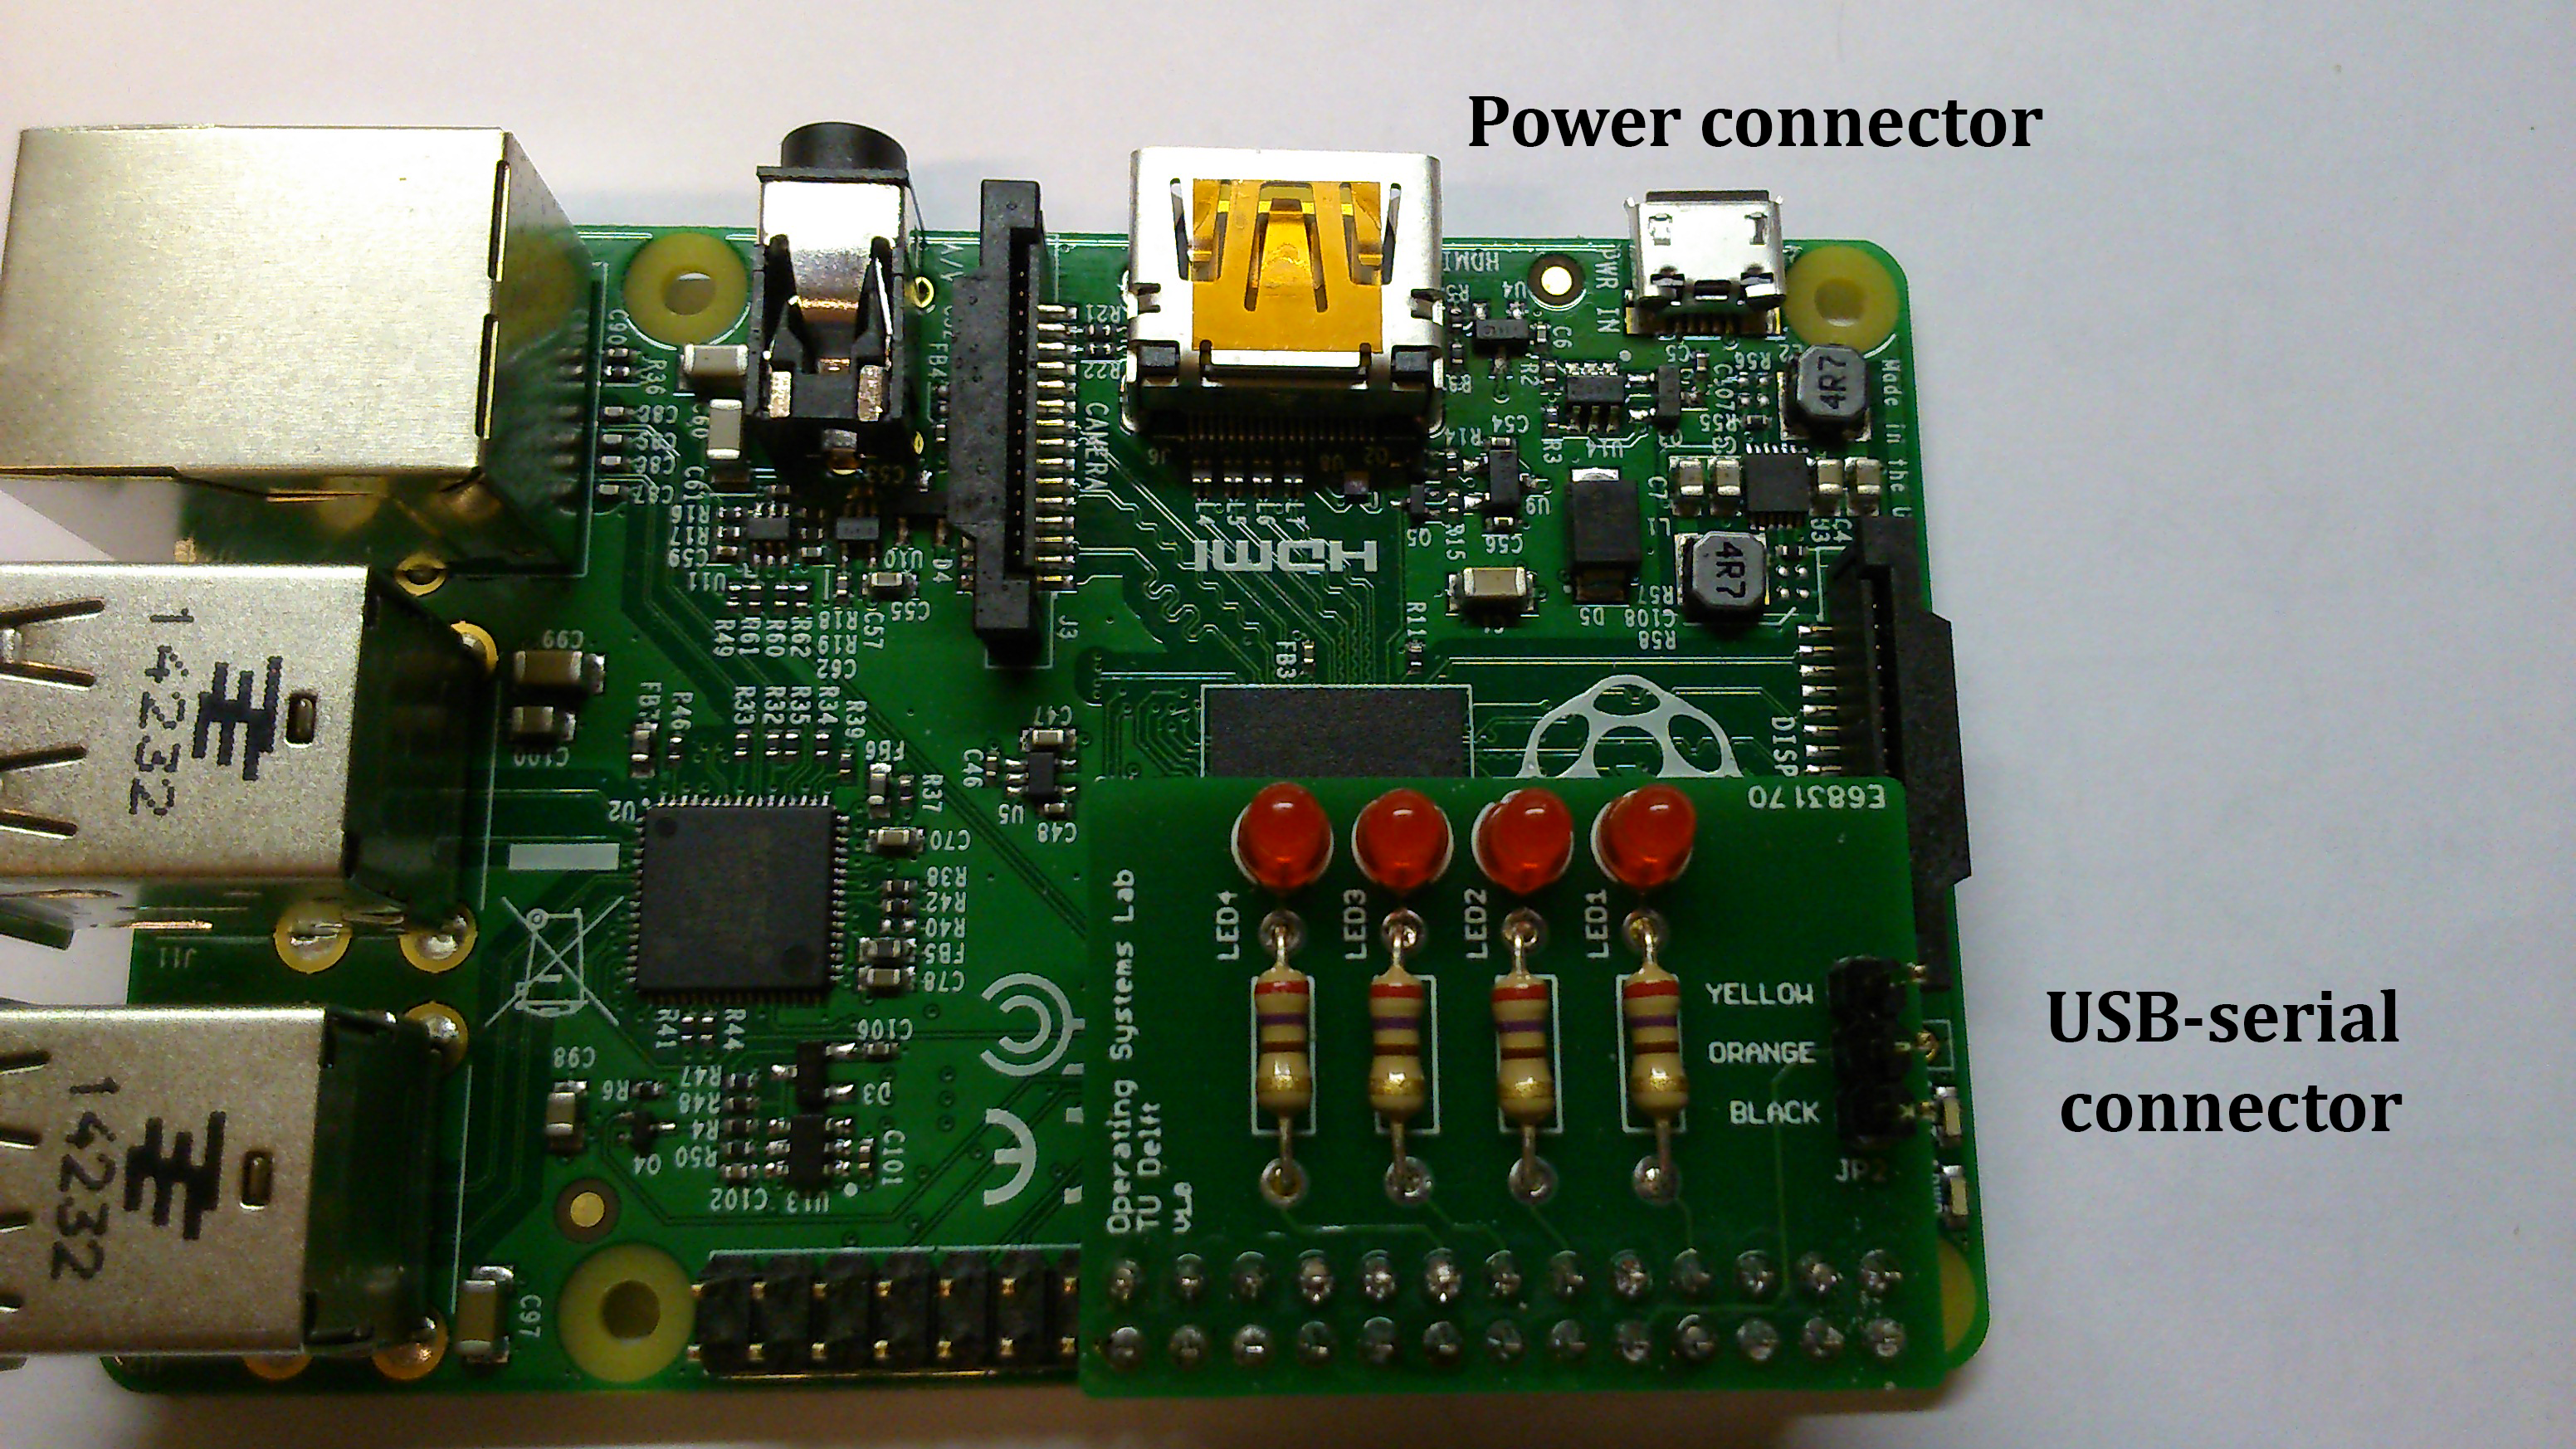
\includegraphics[width=0.80\textwidth]{images/setup.png}
	\caption{Raspberry Pi with extension board}
	\label{fig:raspberry-setup}
\end{figure}


\section{Programming Environment}
\label{sec:environment}
In order to successfully program the supplied hardware, you need an operating system with a compiler. Dozens operating systems exists, however to guarantee functionality and service we will only support the operating systems mentioned below. Please feel free to chose either of these operating systems.

\subsection*{Windows}
As mentioned before you will be using a serial cable as a connecting gateway between the computer and raspberry pi. In the case you are using your own windows powered laptop, it is necessary to install the corresponding drivers. In that case - if you have not already done so - install the PL2303 drivers. These can be downloaded from: \url{http://www.prolific.com.tw/US/ShowProduct.aspx?p_id=225&pcid=41}\\

Follow the steps mentioned on that page to install the driver. The driver is installed in such a way that when you later plug in the USB console lead, it will still launch the ``Found New Hardware'' wizard. If you allow the Wizard to search the Internet and install the drivers, it should work. When you have successfully installed the drivers you will be able to connect to your Raspberry Pi through the Console Lead.\\ 

Before you are able to connect to the device, you need to know to which communication port the Raspberry Pi is connected. You can find this by looking in the \menu{Ports} section of the \menu{Windows Device Manager} which is accessible through \menu{Control Panel} under \menu{System}.\\

The program you need to use for connecting with the Raspberry Pi is called Putty. You can download putty from the website \url{http://www.putty.org}. If you are using an x86 machine you can directly download putty via \url{http://goo.gl/BgbXpy}. It should be noted that Putty is not an installer but the actual program itself. Therefore, no installation is required to run Putty.\\
\begin{figure}[!htbp]
	\centering
		\includegraphics[width=0.80\textwidth]{images/putty-config.jpg}
	\caption{Example configuration for Putty}
	\label{fig:putty-config}
\end{figure}

When you open Putty you have to select the connection type \signal{Serial} from the radio buttons and set the speed to \signal{115200} and the serial line to the com port number you found in the previous paragraph. Additionally, please see figure \ref{fig:putty-config}. If the setup is correct you can open the connection and a console screen will be opened (see figure \ref{fig:console-windows}). Here you have to login with username \menu{pi} and password \menu{raspberry}.

\begin{figure}[!htbp]
	\centering
		\includegraphics[width=0.80\textwidth]{images/console-windows.jpg}
	\caption{Console screen on Windows PC}
	\label{fig:console-windows}
\end{figure}

\subsection*{Linux}
If you use Linux it is not needed to install additional software as the \signal{screen} package is included. However in some Linux distributions such as Ubuntu 12.10, the \signal{screen} package is not included. In this case you will have to install the package. You can do this by typing the following command.

\begin{flushleft}
	\code{sudo apt-get install screen}
\end{flushleft}

In order to find to which TTY port the Raspberry Pi is connected, execute the following command:

\begin{flushleft}
    \code{dmesg | grep tty}
\end{flushleft}

Now if you want to connect to the Raspberry Pi (in this case connected to /dev/ttyUSBO as found in the previous step) you type the following command.

\begin{flushleft}
	\code{screen /dev/ttyUSB0 115200}
\end{flushleft}

When your connection is successfully initialised you will see the screen of figure \ref{fig:console-linux}.

\begin{figure}[!htbp]
	\centering
		\includegraphics[width=0.80\textwidth]{images/console-linux.jpg}
	\caption{Console screen Linux}
	\label{fig:console-linux}
\end{figure}
